% This is based on the LLNCS.DEM the demonstration file of
% the LaTeX macro package from Springer-Verlag
% for Lecture Notes in Computer Science,
% version 2.4 for LaTeX2e as of 16. April 2010
%
% See http://www.springer.com/computer/lncs/lncs+authors?SGWID=0-40209-0-0-0
% for the full guidelines.
%
\documentclass{llncs}

\usepackage{graphicx}
\usepackage{verbatim}
\usepackage{fancyhdr}
\usepackage{listings}
\usepackage{color}

\definecolor{dkgreen}{rgb}{0,0.6,0}
\definecolor{gray}{rgb}{0.5,0.5,0.5}
\definecolor{mauve}{rgb}{0.58,0,0.82}

\lstset{frame=tb,
  language=Prolog,
  aboveskip=3mm,
  belowskip=3mm,
  showstringspaces=false,
  columns=flexible,
  basicstyle={\small\ttfamily},
  numbers=none,
  numberstyle=\tiny\color{gray},
  keywordstyle=\color{blue},
  commentstyle=\color{dkgreen},
  stringstyle=\color{mauve},
  breaklines=true,
  breakatwhitespace=true,
  tabsize=3
  }

\begin{document}

\title{Skyscraper}
%
\titlerunning{Skyscraper}  % abbreviated title (for running head)
%                                     also used for the TOC unless
%                                     \toctitle is used
%
\author{André Cruz\inst{1} \and Edgar Carneiro\inst{2}}
%
\authorrunning{André Cruz \and Edgar Carneiro} % abbreviated author list (for running head)
%
%%%% list of authors for the TOC (use if author list has to be modified)
\tocauthor{André Cruz and Edgar Carneiro}
%
\institute{Faculdade de Engenharia da Universidade do Porto\\ Rua Roberto Frias, sn, 4200-465 Porto, Portugal,\\
\email{ feup@fe.up.pt},\\ WWW home page:
\texttt{http://www.fe.up.pt}}

\maketitle              % typeset the title of the contribution

\begin{abstract}
This article was written for the course unit ``Logic Programming'', from the course Master in Informatics and Computing Engineering.
This article purpose is to present how the program we developed is able to solve the decision problem that is the puzzle Skyscraper, independently of the booard size.
The program developed is also able to generate Skycraper puzzles as well. The program develop uses Logic Programming with Constraints as the approach to solve and generate the puzzles.
\keywords{skycraper, CLP, sicstus, PLOG, FEUP}
\end{abstract}
%
\section{Introduction}
%
The main purpose of this project was to develop a program that would be able to solve either Decision Problems or Otimization Problems, by using Logic Programming with Constraints.

Our group was assigned with a decision problem: the Skyscraper puzzle. Succintly, the puzzle consists of a grid that the player needs to fill, acordding to some given restrictions, and without repeting the same digits per column and per row.

The article approaches several thematics such as: what were the variables used and its domains, what were the constraints used and their implementation in the program, what is the labeling strategy implemented, what are the results of the developed program and what are the final conclusions obtained from developing the project and its pros.

%
\section{Problem Description}
%
Skyscraper consists of a puzzle where the player needs to fill a grid with digits from 1 to \textit{N} --- with \textit{N} being the the size of the grid --- where each row and column contains each digit exactly once. In the grid, each number represents the height of a building. The numbers outside the grid indicate how many buildings can be seen when looking from that direction. Taller buildings block the view of smaller buildiings, meaning that every number, when looking from that direction, beyond a number bigger than it, will not be taken into account.

The difficulty of the puzzle arises from the conjugation of two factors: the digits in rows and columns must all be distinct and the restrictions outside the grid.

\begin{figure}[h!]
\begin{center}
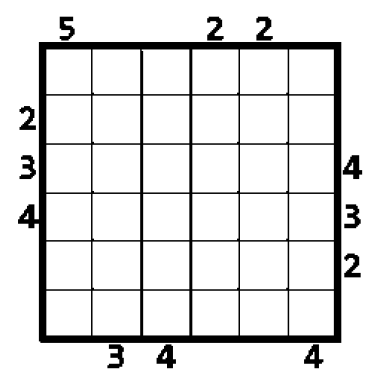
\includegraphics[height=6cm,width=6cm]{images/skyscraper_unsolved.png}
\caption{Unsolved 6x6 Skyscraper puzzle}
\label{Figure 1}
\end{center}
\end{figure}

\begin{figure}[h!]
\begin{center}
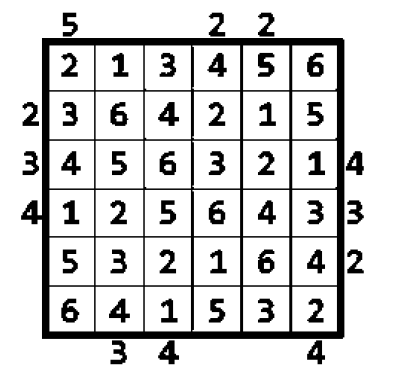
\includegraphics[height=6cm,width=6cm]{images/skyscraper_solved.png}
\caption{Solved 6x6 Skyscraper puzzle}
\label{Figure 2}
\end{center}
\end{figure}

%
\section{Approach}

In the implementation of Scyscraper in Prolog, the group used a list of lists to represent the grid. The value of each element will correspond to the height of the building it represents.
Elements whose value is not known will be represented by  a `\_', therefore representing in Prolog non instantiated values.

For the restrictions outside the grid, the group also decided to use a list of lists.The list containing the other lists will always have length four since each one of its elements is a list containg the restrictions of the correspondent border. The order by which the the border's restricitons are kept in the list is: Top border restrictions, Left border restrictions, Bottom border restrictions and Right border restrictions. If the restriction for a certain row or column does not exist, a `0' is used in its representation.

\begin{figure}[h!]
\begin{center}
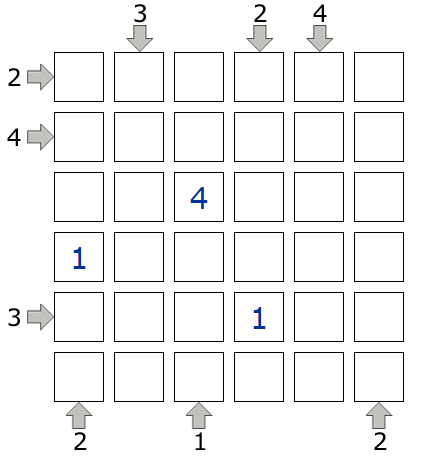
\includegraphics[height=6cm,width=6cm]{images/example_skyscraper.png}
\caption{Example of a skyscrapper puzzle followed by its Prolog representation}
\label{Figure 3}
\end{center}
\end{figure}
\noindent\begin{minipage}{.48\textwidth}
\begin{lstlisting}[frame=tlrb, caption=Prolog grid representation]
testBoard([
  [_, _, _, _, _, _],
  [_, _, _, _, _, _],
  [_, _, 4, _, _, _],
  [1, _, _, _, _, _],
  [_, _, _, 1, _, _],
  [_, _, _, _, _, _]
]).
\end{lstlisting}
\end{minipage}\hfill
\begin{minipage}{.42\textwidth}
\begin{lstlisting}[frame=tblr, caption=Prolog representation of border restrictions]
testRestrictions([
  [0, 3, 0, 2, 4, 0],
  [2, 4, 0, 0, 3, 0],
  [2, 0, 1, 0, 0, 2],
  [0, 0, 0, 0, 0, 0]
]).
\end{lstlisting}
\end{minipage}\hfill

%
\subsection{Decision Variables}

The decision variables associated with a skycraper puzzle are: the lists representing the rows of the grid. Since all the elements in a row and column must have a differente value --- as it is a skycscraper rule --- the domain of the elements in each row will have to be defined between 1 and the length of the board, \textit{N}, and they will also have to be all distinct. The following code presents the application of the referred restrains to the decision variables.\\

\noindent\begin{minipage}{.44\textwidth}
\begin{lstlisting}[frame= tblr, caption=Row domain restrictions]
restrictBoardDomain([], _).
restrictBoardDomain([Row | Board], N) :-
  length(Row, N),
  domain(Row, 1, N),
  all_distinct(Row),
  restrictBoardDomain(Board, N).
\end{lstlisting}
\end{minipage}\hfill
\begin{minipage}{.5\textwidth}
\begin{lstlisting}[frame=tblr, caption=Column all elelemnts distinct]
all_distinct_columns(_, 0) :- !.
all_distinct_columns(Board, N) :-
  N > 0, !,
  getBoardCol(Board, N, Col),
  all_distinct(Col),
  NewN is N - 1,
  all_distinct_columns(Board, NewN).
\end{lstlisting}
\end{minipage}\hfill

\textbf{TODO} Os side domains tb sao? penso que nao porque nao queremos instanciar nada ai... although it seems in code

%
\subsection{Constraints}

The restrictions defined for the puzzle are the ones form the rules. The rules that force the inexistence of repeated elements in either a row or a column were already implemented, by the way the domains are defined (see section \textbf{Decision Variables}). Therefore, the challenge envolving the project was the addition of PROLOG restrictions to implement the missing rule: assuring that the number outside the grid would indeed control the number of `visible buildings'.\textbf{TODO - Ver esta frase, if we did} In the end, some restricitons were also added in order to increase the efficiency of the implemented solution.\\

Theoretically, what we needed to implement in order to achieve the last rule was an IF CLAUSE, being that: if the element is bigger than the maximum value so far, than the element is the new maximum value, and the elemts correspondent building is visible, otherwise, the building is not visible and the maximum value stays the same. However, since in Constraints  Logic Programming the elements value would not be instantiated this implementation proved hard. \textbf{Um bcd bullshit este texto, mudar? xD ou mm apagar}

The solution we came up to implement that last rule was a \textit{logic OR}, because the element being analysed was either a maximum value and the number of visible buildings would increment, or it was not and the count of visible buildings would stay the same. In the end, we wanted to, when the line was finished being analysed, the number of visible buildings would be equal to the corresponding border restraining value. The predicate would be called for each line/ column for each of the four possible directions: left to right, right to left, top to bottom and bottom to top. 

\begin{lstlisting}[frame=tblr, caption=Constraint that assures correct number of visible buildings ]
/**
 * Apply restrictions to Row.
 * +Predicate Order in which elements are analyzed - fetches an element.
 * +Num is the number of visible skyscrapers according to the above order.
 */
applyToRow(Num, Row, Max, GetElement) :-
  call(GetElement, Row, El, RemainderRow),
  NewNum #>= 0,
  (El #> Max #/\ NewMax #= El #/\ NewNum #= Num - 1) #\/
  (El #=< Max #/\ NewMax #= Max #/\ NewNum #= Num),
  applyToRow(NewNum, RemainderRow, NewMax, GetElement).
applyToRow(0, [], _, _).
\end{lstlisting}

\textbf{TODO?  `restrições rígidas e flexíveis' - n encontrei nada sobre isto em pdfs ou lado algum, perguntei e tb nao arranjei quem soubesse. caguei e meti so restrições por geral}

%
\subsection{Evaluation Function}

In Skyscraper there is no evaluation of solutions, since the puzzle is solved whenever a solution is found.

%
\subsection{Search Strategy}

The labeling strategy implemented in the program was the \textbf{\textit{ffc}}, also known as \textit{most\_constrained}. This labeling strategy makes use of the most constrained heuristic: ` a variable with the smallest domain is selected, breaking ties by (a) selecting the variable that has the most constraints suspended on it and (b) selecting the leftmost one.' \textbf{Meter aqui citação} We opted for this heuristic as it would be the one providing faster and more efficient solutions for the skyscraper puzzle. This natural having in mind the kind of constraints that were applied during the development, namely the assure the building heghts were correct.

%
\section{Solution Presentation}

For the solution presentation in text mode the predicate printBoard is used. If run as \textbf{\textit{printBoard(+Board)}}, it only prints the given board in a user friendly way. However, if run as \textbf{\textit{printBoard(+Board, +Restrictions)}} it will print the board in a user friendly way while also displaying the boarder restrictions being applied to each row or column. The predicate makes use of helper predicates such as \textbf{\textit{printRow(+Row)}}, that prints the given row; \textbf{Adicionar aqui mais depois de alturar o codigo buba}. All this predicates are defined in the file \textbf{\textit{display.pl}}.

\textbf{TODO METER AQUI OS PRINTS DEPOIS DAS ALTERAÇÕES}

%
\section{Results}

\textbf{TODO primeiro tetntar otimizar senao os valores que estao aqui serao em vao}

The group tried to make extensive and exhaustive tests, in order to be able to conclude fiercely about the given results.

In the end, the conclusions the group came up with were:
\begin{itemize}
	\item Conclusion 1
	\item Conclusion 2
	\item Conclusion 3 \dots
\end{itemize}

%
\section{Conclusion and Future Work}

We believe that our knowledge about Logic Programming was deeply increased, with everything we had proposed to do being accomplished in the required time.

The program developed has no limitations regarding board size or problem generation, despite becoming slower with bigger board sizes. Therefore, the only way possible to improve the developed application would be by improving the solver efficiency and time. However, the group tried fiercely to make that improve by trying out several approaches but in the end, the best solution was the one being presented.

The group also agreed in the fact that Logic Programming with Constrains revealed itself to be an extremelly powerful tool, able to solve easily certain problems (such as the one this work is based in) that woudl take much more time and effort to solve with other paradgims.\\

To sum up, despite Logic Programming with Constrainsts being a totally different paradgim drom what the group had ever worked with, we quickly got used to it and learnt to appreciate the cons and pros that it presents, thus having it culimante in a project we are proud of.

%


%
% ---- Bibliography ----
%
\begin{thebibliography}{5}
%
\bibitem {ster:shap:warr}
L. Sterling, E. Y. Shapiro, and D. H. D. Warren, The Art of Prolog: Advanced Programming Techniques. MIT Press, 2010.

\bibitem {carl:fru}
M. Carlsson and T. Fruhwirth, SICStus Prolog User's Manual. SICS Swedish ICT AB, 4.3.5 ed., 2016.

\bibitem {sky}
Skyscraper rules,
http://logicmastersindia.com/lmitests/dl.asp?attachmentid=659\&view=1

\end{thebibliography}

\appendix

\end{document}
